\documentclass[a4paper]{article}\usepackage{graphicx, color}
%% maxwidth is the original width if it is less than linewidth
%% otherwise use linewidth (to make sure the graphics do not exceed the margin)
\makeatletter
\def\maxwidth{ %
  \ifdim\Gin@nat@width>\linewidth
    \linewidth
  \else
    \Gin@nat@width
  \fi
}
\makeatother

\IfFileExists{upquote.sty}{\usepackage{upquote}}{}
\definecolor{fgcolor}{rgb}{0.2, 0.2, 0.2}
\newcommand{\hlnumber}[1]{\textcolor[rgb]{0,0,0}{#1}}%
\newcommand{\hlfunctioncall}[1]{\textcolor[rgb]{0.501960784313725,0,0.329411764705882}{\textbf{#1}}}%
\newcommand{\hlstring}[1]{\textcolor[rgb]{0.6,0.6,1}{#1}}%
\newcommand{\hlkeyword}[1]{\textcolor[rgb]{0,0,0}{\textbf{#1}}}%
\newcommand{\hlargument}[1]{\textcolor[rgb]{0.690196078431373,0.250980392156863,0.0196078431372549}{#1}}%
\newcommand{\hlcomment}[1]{\textcolor[rgb]{0.180392156862745,0.6,0.341176470588235}{#1}}%
\newcommand{\hlroxygencomment}[1]{\textcolor[rgb]{0.43921568627451,0.47843137254902,0.701960784313725}{#1}}%
\newcommand{\hlformalargs}[1]{\textcolor[rgb]{0.690196078431373,0.250980392156863,0.0196078431372549}{#1}}%
\newcommand{\hleqformalargs}[1]{\textcolor[rgb]{0.690196078431373,0.250980392156863,0.0196078431372549}{#1}}%
\newcommand{\hlassignement}[1]{\textcolor[rgb]{0,0,0}{\textbf{#1}}}%
\newcommand{\hlpackage}[1]{\textcolor[rgb]{0.588235294117647,0.709803921568627,0.145098039215686}{#1}}%
\newcommand{\hlslot}[1]{\textit{#1}}%
\newcommand{\hlsymbol}[1]{\textcolor[rgb]{0,0,0}{#1}}%
\newcommand{\hlprompt}[1]{\textcolor[rgb]{0.2,0.2,0.2}{#1}}%

\usepackage{framed}
\makeatletter
\newenvironment{kframe}{%
 \def\at@end@of@kframe{}%
 \ifinner\ifhmode%
  \def\at@end@of@kframe{\end{minipage}}%
  \begin{minipage}{\columnwidth}%
 \fi\fi%
 \def\FrameCommand##1{\hskip\@totalleftmargin \hskip-\fboxsep
 \colorbox{shadecolor}{##1}\hskip-\fboxsep
     % There is no \\@totalrightmargin, so:
     \hskip-\linewidth \hskip-\@totalleftmargin \hskip\columnwidth}%
 \MakeFramed {\advance\hsize-\width
   \@totalleftmargin\z@ \linewidth\hsize
   \@setminipage}}%
 {\par\unskip\endMakeFramed%
 \at@end@of@kframe}
\makeatother

\definecolor{shadecolor}{rgb}{.97, .97, .97}
\definecolor{messagecolor}{rgb}{0, 0, 0}
\definecolor{warningcolor}{rgb}{1, 0, 1}
\definecolor{errorcolor}{rgb}{1, 0, 0}
\newenvironment{knitrout}{}{} % an empty environment to be redefined in TeX

\usepackage{alltt}
\usepackage{geometry}
\usepackage{float}
\usepackage{longtable}
\usepackage{amsmath}
\usepackage[bottom]{footmisc}
\usepackage{amssymb}
\usepackage{graphicx}
\usepackage{cite}
\usepackage{color} 
\usepackage{setspace} 
\usepackage[labelfont=bf,labelsep=period,justification=raggedright]{caption}
\geometry{verbose,a4paper,tmargin=3cm,bmargin=2cm,lmargin=2cm,rmargin=3cm}
\setlength{\parskip}{\medskipamount}
\setlength{\parindent}{0pt}
\bibliographystyle{plos2009}

\begin{document}
\title{a4a assessment model simulation testing}
\author{Jardim, E., Millar, C., Ferretti, M., Mosqueira, I., Osio, C. and Scott, F.}
%\affiliations{Maritime Affairs unit, Institute for the Protection and Security of the Citizen, European Commission Joint Research Centre, Ispra, Varese, Italy}

\maketitle
\pagebreak
\tableofcontents
\pagebreak

\newpage
\section{Introduction}

Simulation testing provides information about the performance of the model in specific circumstances, which is a major source of information for analysts. Informing about regions of the parameters space that may require more attention in order to overcome problems that surfaced during testing phase. Simulation testing \emph{Per se} does not cover the full range of situations that may occur, these are a lot wider than it's possible to simulate. The simulation environment does allow a controlled experiment to be carried out which gives information about the capacity of the model to reconstruct the underlying reality under specific conditions. Furthermore, these simulation studies allows testing the adjustment of models without much human intervention (automatic adjustments), a major objective of the framework developed here.

To run the simulation study the following algorithm was applied:
\begin{enumerate}
	\item Use information about life history traits of several fish stocks to build coherent population dynamics under no-exploitation scenario.
	\item Simulate for each stock a 50 year exploitation history based on the common development-over exploitation-recovery pattern.
	\item Trim the simulations in four 15 year periods, generating a range of exploitation patterns that are commonly observed in global fisheries: (i) "development" - from non-exploited fisheries up to over-exploitation, (ii) "development plus over-exploitation" - five years of increasing fishing mortality and 10 years of over-exploitation, (iii) "over-exploitation" - 15 years of stable fishing mortality at over-exploitation levels, and (iv) "recovery" - 5 years of over-exploitation and 10 years decreasing fishing mortality down to the maximum sustainable yield (MSY) fishing mortality.
	\item Add observation error in abundance indices considering several assumptions about catchability and independent lognormal errors with several levels of variability.
	\item Add observation error in catch in numbers at age in the form of independent lognormal errors with several levels of variability.
	\item Fit a random assessment model to each simulation by selecting the sub-models from a set of three distinct F models, five distinct Q models and two distinct R models.
	\item Compute performance statistics.
\end{enumerate}

The approach taken regarding the population dynamics does not try to simulate exactly specific species, it aims to simulate stocks and exploitation histories that are consistent with population dynamics theory and loosely based on the biology of the species, so that a large range of life histories traits and commercial exploitation patterns are considered.     

For this simulation exercise, life history parameters were extracted from FishBase \cite{froesefishbase2013} for all marine species available. Over-exploitation was defined by fishing levels of 80\% of the crash fishing mortality \cite{quinn1999quantitative} or five times the level of F$_{0.1}$ \cite{gullandF0.1}. 

The results were integrated in an on-line application, using a database and a visualization tool that allows the users to search and download subsets of the data, as well as visualizing directly the performance for particular scenarios. Instead of presenting a massive amount of analysis in this paper the information can be easily analysed on-line or extracted. The information can be used to evaluate the performance of the model, but it can also be used as a starting point to carry out stock assessments, learn how to use the framework, etc. Ultimately it shows that it is possible to run a massive number of stock assessments and make the results available and manageable for those interested in meta analysis. 

Note that all the analysis are carried out in R\footnote{R Core Team ...}, using the FLR\footnote{Kell et. al} libraries and the a4a package for the stock assessment model. The document is written in LaTeX using the R package knitr\footnote{REF}, which embeds the code in the document. The major advantage is allowing full replicability of the analysis and readers to check the code.

This document is supplemental material to the paper Colin, et.al (2013) and shows the scenarios and code used for the simulation study 1.

\section{Webscrap fishbase}

\begin{knitrout}
\definecolor{shadecolor}{rgb}{0.969, 0.969, 0.969}\color{fgcolor}\begin{kframe}


{\ttfamily\noindent\bfseries\color{errorcolor}{\#\# Error: there is no package called 'FLAdvice'}}

{\ttfamily\noindent\bfseries\color{errorcolor}{\#\# Error: no existing definition for function 'sv'}}\end{kframe}
\end{knitrout}


\begin{knitrout}
\definecolor{shadecolor}{rgb}{0.969, 0.969, 0.969}\color{fgcolor}\begin{kframe}
\begin{alltt}
\hlfunctioncall{library}(FLCore)
\hlfunctioncall{library}(FLAdvice)
\hlfunctioncall{library}(rfishbase)
\hlfunctioncall{library}(longtable)
\hlfunctioncall{library}(XML)
fish.data <- \hlfunctioncall{loadCache}()

\hlcomment{# ============================================================}
\hlcomment{#' extract information in rfishbase}
\hlcomment{# ============================================================}
ids <- \hlfunctioncall{unlist}(\hlfunctioncall{lapply}(fish.data, \hlstring{"["}, \hlstring{"id"}))
order <- \hlfunctioncall{unlist}(\hlfunctioncall{lapply}(fish.data, \hlstring{"["}, \hlstring{"Order"}))
family <- \hlfunctioncall{unlist}(\hlfunctioncall{lapply}(fish.data, \hlstring{"["}, \hlstring{"Family"}))
spp <- \hlfunctioncall{unlist}(\hlfunctioncall{lapply}(fish.data, \hlstring{"["}, \hlstring{"ScientificName"}))
maxage <- \hlfunctioncall{getSize}(fish.data, \hlstring{"age"})
maxlen <- \hlfunctioncall{getSize}(fish.data, \hlstring{"length"})
maxwgt <- \hlfunctioncall{getSize}(fish.data, \hlstring{"weight"})
mar <- \hlfunctioncall{vector}(\hlstring{"logical"}, length = \hlfunctioncall{length}(ids))
mar[\hlfunctioncall{grep}(\hlstring{"marine"}, \hlfunctioncall{unlist}(\hlfunctioncall{lapply}(fish.data, \hlstring{"["}, \hlstring{"habitat"})))] <- TRUE

\hlcomment{# ============================================================}
\hlcomment{#' init results dataframe with data from rfishbase}
\hlcomment{# ============================================================}
lhPars <- \hlfunctioncall{data.frame}(id = ids, order = order, family = family, species = spp, 
    marine = mar, a = NA, b = NA, k = NA, linf = NA, t0 = NA, a50 = NA, l50 = NA, 
    lmax = maxlen, amax = maxage, wmax = maxwgt, stringsAsFactors = FALSE)

\hlcomment{# ============================================================}
\hlcomment{#' scrap}
\hlcomment{# ============================================================}
\hlfunctioncall{for} (i in ids) \{
    \hlfunctioncall{cat}(i, \hlstring{";"})
\hlcomment{    # --------------------------------------------------------}
\hlcomment{    #' growth}
\hlcomment{    # --------------------------------------------------------}
    addr <- \hlfunctioncall{paste}(\hlstring{"http://www.fishbase.org/PopDyn/PopGrowthList.php?ID="}, i, 
        sep = \hlstring{""})
    tab <- \hlfunctioncall{try}(\hlfunctioncall{readHTMLTable}(addr))
    \hlfunctioncall{if} (\hlfunctioncall{is}(tab, \hlstring{"try-error"})) 
        tab$dataTable <- NULL
    \hlfunctioncall{if} (!\hlfunctioncall{is.null}(tab$dataTable)) \{
\hlcomment{        # linf}
        v <- \hlfunctioncall{as.character}(tab$dataTable[, \hlstring{"\hlfunctioncall{Loo}(cm)"}])
        \hlfunctioncall{for} (j in 1:\hlfunctioncall{length}(v)) \{
            vj <- v[j]
            vj <- \hlfunctioncall{utf8ToInt}(vj)
            v[j] <- \hlfunctioncall{intToUtf8}(vj[vj >= 46 & vj <= 57])
        \}
        lhPars[lhPars$id == i, \hlstring{"linf"}] <- \hlfunctioncall{median}(\hlfunctioncall{as.numeric}(v), na.rm = T)
\hlcomment{        # k}
        v <- \hlfunctioncall{as.character}(tab$dataTable[, \hlstring{"\hlfunctioncall{K}(1/y)"}])
        \hlfunctioncall{for} (j in 1:\hlfunctioncall{length}(v)) \{
            vj <- v[j]
            vj <- \hlfunctioncall{utf8ToInt}(vj)
            v[j] <- \hlfunctioncall{intToUtf8}(vj[vj >= 46 & vj <= 57])
        \}
        lhPars[lhPars$id == i, \hlstring{"k"}] <- \hlfunctioncall{median}(\hlfunctioncall{as.numeric}(v), na.rm = T)
\hlcomment{        # t0}
        v <- \hlfunctioncall{as.character}(tab$dataTable[, \hlstring{"\hlfunctioncall{to}(years)"}])
        \hlfunctioncall{for} (j in 1:\hlfunctioncall{length}(v)) \{
            vj <- v[j]
            vj <- \hlfunctioncall{utf8ToInt}(vj)
            v[j] <- \hlfunctioncall{intToUtf8}(vj[vj >= 46 & vj <= 57])
        \}
        lhPars[lhPars$id == i, \hlstring{"t0"}] <- \hlfunctioncall{median}(\hlfunctioncall{as.numeric}(v), na.rm = T)
    \}
\hlcomment{    # --------------------------------------------------------}
\hlcomment{    #' maturity}
\hlcomment{    # --------------------------------------------------------}
    addr <- \hlfunctioncall{paste}(\hlstring{"http://www.fishbase.org/Reproduction/MaturityList.php?ID="}, 
        i, sep = \hlstring{""})
    tab <- \hlfunctioncall{try}(\hlfunctioncall{readHTMLTable}(addr))
    \hlfunctioncall{if} (\hlfunctioncall{is}(tab, \hlstring{"try-error"})) 
        tab$dataTable <- NULL
    \hlfunctioncall{if} (!\hlfunctioncall{is.null}(tab$dataTable)) \{
\hlcomment{        # l50}
        v <- \hlfunctioncall{as.character}(tab$dataTable[, \hlstring{"\hlfunctioncall{Lm}(cm)"}])
        \hlfunctioncall{for} (j in 1:\hlfunctioncall{length}(v)) \{
            vj <- v[j]
            vj <- \hlfunctioncall{utf8ToInt}(vj)
            v[j] <- \hlfunctioncall{intToUtf8}(vj[vj >= 46 & vj <= 57])
        \}
        lhPars[lhPars$id == i, \hlstring{"l50"}] <- \hlfunctioncall{median}(\hlfunctioncall{as.numeric}(v), na.rm = T)
\hlcomment{        # a50}
        v <- \hlfunctioncall{as.character}(tab$dataTable[, 8])
        \hlfunctioncall{for} (j in 1:\hlfunctioncall{length}(v)) \{
            vj <- v[j]
            vj <- \hlfunctioncall{utf8ToInt}(vj)
            v[j] <- \hlfunctioncall{intToUtf8}(vj[vj >= 46 & vj <= 57])
        \}
        lhPars[lhPars$id == i, \hlstring{"a50"}] <- \hlfunctioncall{median}(\hlfunctioncall{as.numeric}(v), na.rm = T)
    \}
\hlcomment{    # --------------------------------------------------------}
\hlcomment{    #' l~w}
\hlcomment{    # --------------------------------------------------------}
    addr <- \hlfunctioncall{paste}(\hlstring{"http://www.fishbase.org/PopDyn/LWRelationshipList.php?ID="}, 
        i, sep = \hlstring{""})
    tab <- \hlfunctioncall{try}(\hlfunctioncall{readHTMLTable}(addr))
    \hlfunctioncall{if} (\hlfunctioncall{is}(tab, \hlstring{"try-error"})) 
        tab$dataTable <- NULL else \hlfunctioncall{names}(tab)[3] <- \hlstring{"dataTable"}
    \hlfunctioncall{if} (!\hlfunctioncall{is.null}(tab$dataTable)) \{
\hlcomment{        # a}
        v <- \hlfunctioncall{as.character}(tab$dataTable[, 2])
        \hlfunctioncall{for} (j in 1:\hlfunctioncall{length}(v)) \{
            vj <- v[j]
            vj <- \hlfunctioncall{utf8ToInt}(vj)
            v[j] <- \hlfunctioncall{intToUtf8}(vj[vj >= 46 & vj <= 57])
        \}
        lhPars[lhPars$id == i, \hlstring{"a"}] <- \hlfunctioncall{median}(\hlfunctioncall{as.numeric}(v), na.rm = T)
\hlcomment{        # b}
        v <- \hlfunctioncall{as.character}(tab$dataTable[, 3])
        \hlfunctioncall{for} (j in 1:\hlfunctioncall{length}(v)) \{
            vj <- v[j]
            vj <- \hlfunctioncall{utf8ToInt}(vj)
            v[j] <- \hlfunctioncall{intToUtf8}(vj[vj >= 46 & vj <= 57])
        \}
        lhPars[lhPars$id == i, \hlstring{"b"}] <- \hlfunctioncall{median}(\hlfunctioncall{as.numeric}(v), na.rm = T)
    \}
\}
\end{alltt}
\end{kframe}
\end{knitrout}


\begin{knitrout}
\definecolor{shadecolor}{rgb}{0.969, 0.969, 0.969}\color{fgcolor}\begin{kframe}
\begin{alltt}
\hlcomment{# ============================================================}
\hlcomment{#' cleaning & replacing missing values}
\hlcomment{# ============================================================}
lhMar <- \hlfunctioncall{subset}(lhPars, marine == TRUE)
lhMar[lhMar == 0] <- NA
\hlcomment{# ------------------------------------------------------------}
\hlcomment{#' remove sea horses}
\hlcomment{# ------------------------------------------------------------}
lhMar01 <- \hlfunctioncall{subset}(lhMar, !(\hlfunctioncall{is.na}(a) | \hlfunctioncall{is.na}(b) | \hlfunctioncall{is.na}(k) | \hlfunctioncall{is.na}(linf)) & order != 
    \hlstring{"Syngnathiformes"})
\hlcomment{# ------------------------------------------------------------}
\hlcomment{#' id those that were observations}
\hlcomment{# ------------------------------------------------------------}
lhMar01$l50obs <- !\hlfunctioncall{is.na}(lhMar01$l50)
lhMar01$a50obs <- !\hlfunctioncall{is.na}(lhMar01$a50)
lhMar01$amaxobs <- !\hlfunctioncall{is.na}(lhMar01$amax)
lhMar01$t0obs <- !\hlfunctioncall{is.na}(lhMar01$t0)
lhMar01 <- \hlfunctioncall{transform}(lhMar01, obs = (l50obs + a50obs + amaxobs + t0obs) > 0)
\end{alltt}
\end{kframe}
\end{knitrout}


\begin{knitrout}
\definecolor{shadecolor}{rgb}{0.969, 0.969, 0.969}\color{fgcolor}\begin{kframe}
\begin{alltt}
\hlcomment{# ============================================================}
\hlcomment{#' estimate missing values for l50, a50 and amax}
\hlcomment{# ============================================================}
rlm01 <- \hlfunctioncall{rlm}(\hlfunctioncall{log}(l50) ~ \hlfunctioncall{log}(linf), data = \hlfunctioncall{subset}(lhMar01, linf < 300))
lhMar01[\hlfunctioncall{is.na}(lhMar01$l50), \hlstring{"l50"}] <- \hlfunctioncall{exp}(\hlfunctioncall{predict}(rlm01, newdata = \hlfunctioncall{data.frame}(linf = lhMar01[\hlfunctioncall{is.na}(lhMar01$l50), 
    \hlstring{"linf"}])) + \hlfunctioncall{rnorm}(\hlfunctioncall{sum}(\hlfunctioncall{is.na}(lhMar01$l50)), 0, \hlfunctioncall{sd}(\hlfunctioncall{residuals}(rlm01))))

rlm02 <- \hlfunctioncall{rlm}(\hlfunctioncall{log}(t0) ~ \hlfunctioncall{log}(k), data = \hlfunctioncall{subset}(lhMar01, linf < 300))
lhMar01[\hlfunctioncall{is.na}(lhMar01$t0), \hlstring{"t0"}] <- \hlfunctioncall{exp}(\hlfunctioncall{predict}(rlm02, newdata = \hlfunctioncall{data.frame}(k = lhMar01[\hlfunctioncall{is.na}(lhMar01$t0), 
    \hlstring{"k"}])) + \hlfunctioncall{rnorm}(\hlfunctioncall{sum}(\hlfunctioncall{is.na}(lhMar01$t0)), 0, \hlfunctioncall{sd}(\hlfunctioncall{residuals}(rlm02))))

rlm03 <- \hlfunctioncall{rlm}(\hlfunctioncall{log}(amax) ~ \hlfunctioncall{log}(linf), data = lhMar01)
lhMar01[\hlfunctioncall{is.na}(lhMar01$amax), \hlstring{"amax"}] <- \hlfunctioncall{exp}(\hlfunctioncall{predict}(rlm03, newdata = \hlfunctioncall{data.frame}(linf = lhMar01[\hlfunctioncall{is.na}(lhMar01$amax), 
    \hlstring{"linf"}])) + \hlfunctioncall{rnorm}(\hlfunctioncall{sum}(\hlfunctioncall{is.na}(lhMar01$amax)), 0, \hlfunctioncall{sd}(\hlfunctioncall{residuals}(rlm03))))

vv <- -\hlfunctioncall{log}(1 - (lhMar01$l50/lhMar01$linf))/lhMar01$k + lhMar01$t0
lhMar01[\hlfunctioncall{is.na}(lhMar01$a50), \hlstring{"a50"}] <- vv[\hlfunctioncall{is.na}(lhMar01$a50)]
\end{alltt}
\end{kframe}
\end{knitrout}





\begin{knitrout}
\definecolor{shadecolor}{rgb}{0.969, 0.969, 0.969}\color{fgcolor}\begin{figure}[H]

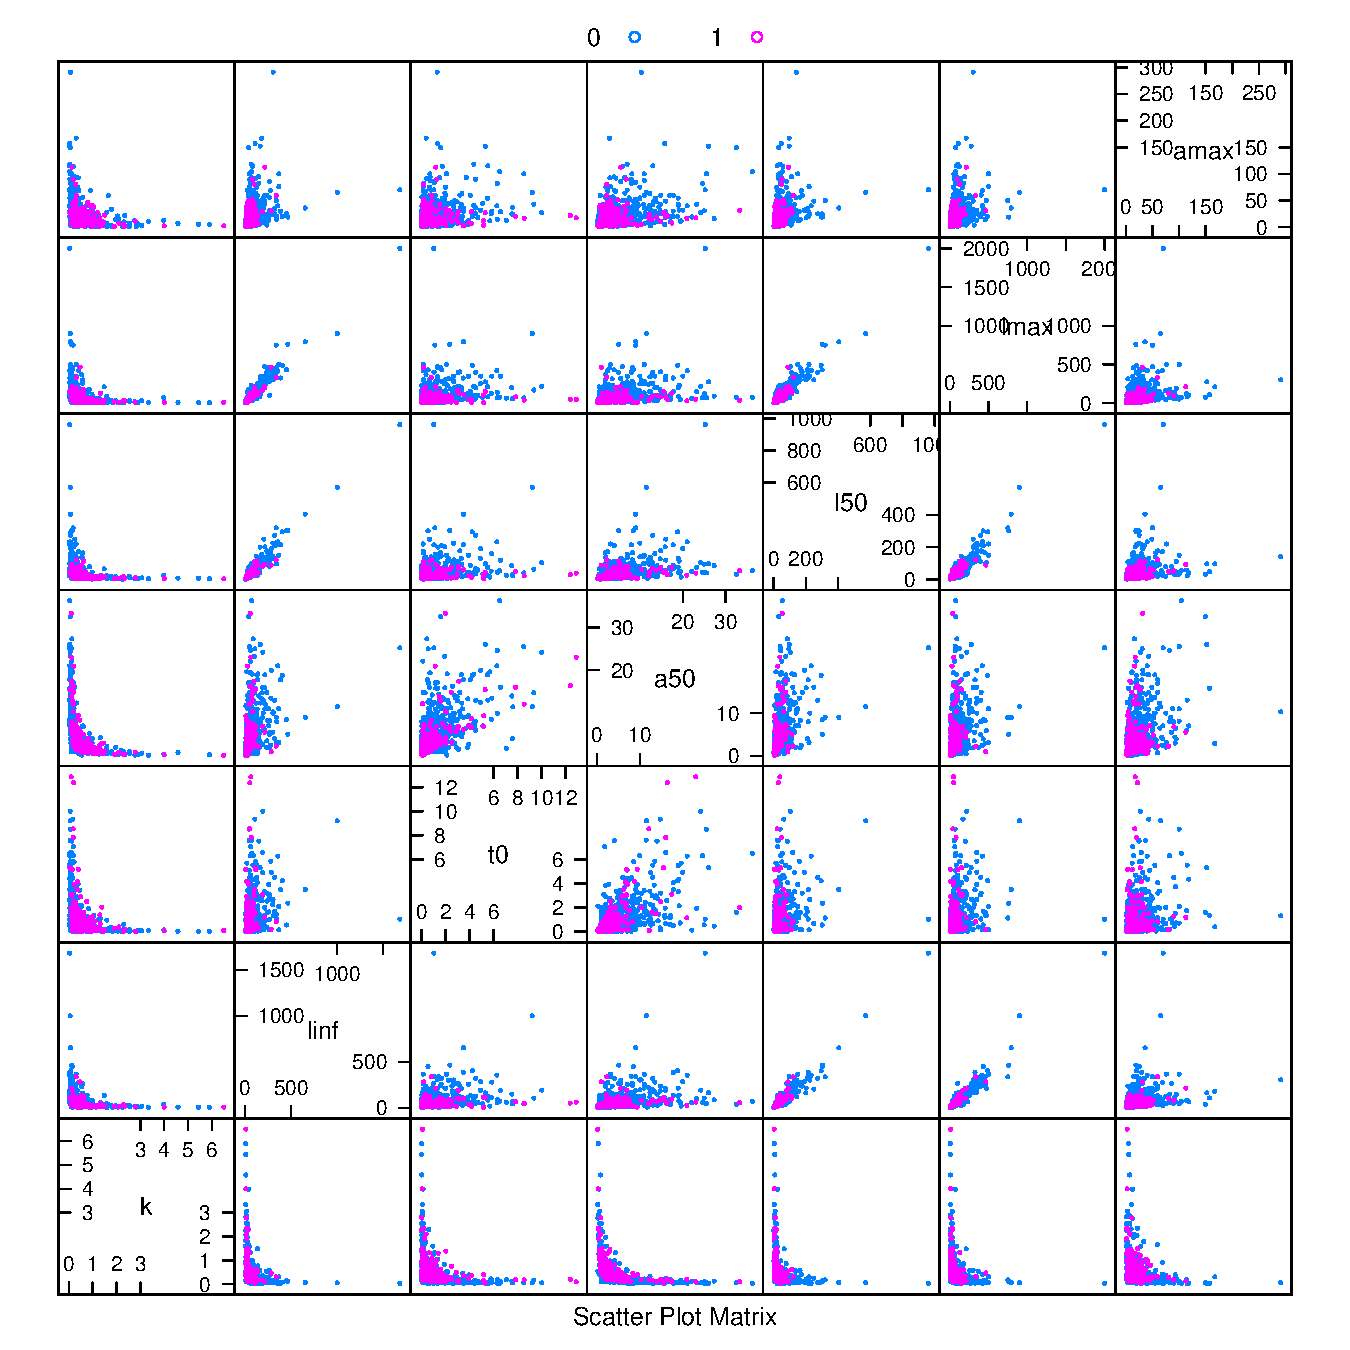
\includegraphics[width=\maxwidth]{figure/unnamed-chunk-6} \caption[Scrapped values and linear model estimates to replace missing values]{Scrapped values and linear model estimates to replace missing values\label{fig:unnamed-chunk-6}}
\end{figure}


\end{knitrout}


\begin{knitrout}
\definecolor{shadecolor}{rgb}{0.969, 0.969, 0.969}\color{fgcolor}\begin{kframe}
\begin{alltt}
\hlcomment{# ------------------------------------------------------------}
\hlcomment{#' variables from fishbase}
\hlcomment{# ------------------------------------------------------------}
\hlfunctioncall{names}(lhMar01)
\end{alltt}
\begin{verbatim}
##  [1] "id"      "order"   "family"  "species" "marine"  "a"       "b"      
##  [8] "k"       "linf"    "t0"      "a50"     "l50"     "lmax"    "amax"   
## [15] "wmax"    "l50obs"  "a50obs"  "amaxobs" "t0obs"   "obs"
\end{verbatim}
\begin{alltt}
\hlcomment{# ------------------------------------------------------------}
\hlcomment{#' number of species}
\hlcomment{# ------------------------------------------------------------}
\hlfunctioncall{nrow}(lhMar01)
\end{alltt}
\begin{verbatim}
## [1] 1053
\end{verbatim}
\end{kframe}
\end{knitrout}


\section{Scenarios}

For each species the following scenarios were simulated.

\begin{knitrout}
\definecolor{shadecolor}{rgb}{0.969, 0.969, 0.969}\color{fgcolor}\begin{kframe}
\begin{alltt}
\hlcomment{# ------------------------------------------------------------}
\hlcomment{#' Operating models}
\hlcomment{# ------------------------------------------------------------}
\hlcomment{#' stock recruitment models}
srMod <- \hlfunctioncall{c}(\hlstring{"bevholt"}, \hlstring{"ricker"})
\hlcomment{#' steepness of stock recruitment relationship}
s <- \hlfunctioncall{c}(0.8, 0.6)
\hlcomment{#' age of 50% selectivity (maximum of double normal model)}
a1 <- \hlfunctioncall{c}(0.7, 1)  \hlcomment{# relative to a50}
\hlcomment{#' variance of the right half of the double normal}
sr <- \hlfunctioncall{c}(1, 100)
\hlcomment{#' variance of the left half of the double normal}
sl <- \hlfunctioncall{c}(1, 100)

\hlcomment{# ------------------------------------------------------------}
\hlcomment{#' Observation error}
\hlcomment{# ------------------------------------------------------------}
\hlcomment{#' coefficient of variation for catch at age lognormal errors}
oe.ccv <- \hlfunctioncall{c}(0.1, 0.3)
\hlcomment{#' coefficient of variation for index at age lognormal errors}
oe.icv <- \hlfunctioncall{c}(0.2, 0.5)
\hlcomment{#' linear increase by year for index catchability}
oe.iq <- \hlfunctioncall{c}(1, 1.05)  \hlcomment{# technical creep, q = 0.01}
\end{alltt}
\end{kframe}
\end{knitrout}





Scenarios with flat selectivity and a1=0.7 were removed once a1 has no effect. Also cases that end up with missing values in the age of 50\% mature fish were removed. Finally the number of scenarios were 224 that when merged with the species and for each combination five exploitation histories were simulated, giving raise to approximately 1.15 million simulations.

\section{Model fit}

Afterwards a set of models were built, considering the most common options used in stock assessment (see below) which generate a total of 30 combinations. For each simulation one of these combinations was allocated randomly to be used in the model fit.




% latex.default(df0, longtable = FALSE, file = "", caption = "Sub-models used for fitting.",      rowname = NULL, where = "H", colheads = c("submodel", "code",          "formula"), first.hline.double = FALSE) 
%
\begin{table}[H]
\caption{Sub-models used for fitting.\label{df0}} 
\begin{center}
\begin{tabular}{lll}
\hline
\multicolumn{1}{c}{submodel}&\multicolumn{1}{c}{code}&\multicolumn{1}{c}{formula}\tabularnewline
\hline
fishery&fm1&~factor(age) + factor(year)\tabularnewline
fishery&fm2&~bs(age, 4) + bs(year, 10)\tabularnewline
fishery&fm3&~te(age, year, bs = c("tp", "tp"), k = c(4, 15))\tabularnewline
catchability&qm0&~1\tabularnewline
catchability&qm1&~age\tabularnewline
catchability&qm2&~factor(age)\tabularnewline
catchability&qm3&~bs(age, 4)\tabularnewline
catchability&qm4&~bs(age, 4) + bs(year, 15)\tabularnewline
recruitment&rm1&~factor(year)\tabularnewline
recruitment&rm2&~bs(year, 15)\tabularnewline
\hline
\end{tabular}
\end{center}
\end{table}




\section{Results}

The results are made available on a dedicated web page on the a4a website. The page accesses a database with all the results and provides visualization and exporting tools.

\subsection{Export file data structure}

The data is split in two tables, "stats" and "summs". The first has summary stats of the tests. Table "stats" is linked one to many with table "summs", which has summaries of the stock assessment fits. Both tables have the field "scnid", which is the scenario identification field. The scenario identification kwy is build by concatenating other fields, which are identified by the string "scnid" in bold. This field can be used to link both tables. 

\subsubsection{Table "stats" fields}

\begin{itemize}
	\item scenario parameters
	\begin{itemize}
		\item order, text, taxon order, 
		\item family, text, taxon family, 
		\item species, text, taxon species, {\bf scnid}
		\item marine, bolean, marine species or not,
		\item a, numeric, parameter of the weight-length relationship,
		\item b, numeric, parameter of the weight-length relationship,
		\item k, numeric, parameter of the von Bertalanffy growth model,
		\item linf, numeric, parameter of the von Bertalanffy growth model,
		\item t0, numeric, parameter of the von Bertalanffy growth model,
		\item a50, numeric, age of 50\% maturity, 
		\item l50, numeric, length of 50\% maturity, 
		\item amax, numeric, maximum age, 
		\item lmax, numeric, maximum length, 
		\item wmax, numeric, maximum weight, 
		\item l50obs, bolean, was l50 observed or not,
		\item a50obs, bolean, was a50 observed or not,
		\item amaxobs, bolean, was amax observed or not,
		\item t0obs, bolean, was t0 observed or not,
		\item obs, ignore,,
		\item srMod, text, stock-recruitment model, {\bf scnid}
		\item s, numeric, steepness parameter of the stock-recruitment curve, {\bf scnid}
		\item v, numeric, virgin biomass parameter of the stock-recruitment curve, {\bf scnid}
		\item a1, numeric, age of 50\% selectivity parameter of the selectivity double normal model, {\bf scnid}
		\item sr, numeric, right variance parameter of the selectivity double normal model, {\bf scnid}
		\item sl, numeric, left variance parameter of the selectivity double normal model, {\bf scnid}
		\item oe.icv, numeric, abundance index coefficient of variation parameter of the observation error model, {\bf scnid}
		\item oe.iq, numeric, abundance index catchability increase parameter of the observation error model, {\bf scnid}
		\item oe.ccv, numeric, catch at age coefficient of variation parameter of the observation error model, {\bf scnid}
		\item qmodel, text, catchability model, {\bf scnid}
		\item rmodel, text, recruitment model, {\bf scnid}
		\item fmodel, text, fishing mortality model, {\bf scnid}
		\item fmsy, numeric, fmsy fishing mortality reference point,
		\item f0.1, numeric, f0.1 fishing mortality reference point,
		\item m, numeric, natural mortality average over age range, 
		\item expl, numeric, exploitation history pattern, {\bf scnid}
	\end{itemize}
	\item fitting statistics
	\begin{itemize}
		\item nopar, numeric, number of model parameters, 
		\item nlogl, numeric, negative log likelihood of the fit,
		\item maxgrad, numeric, maximum gradient of the negative log likelihood surface,
		\item npar, ignore,, 
		\item logDetHess, ignore,,
	\end{itemize}
	\item comparison statistics
	\begin{itemize}
		\item ssbrbias, numeric, SSB relative bias, 
		\item ssbmse, numeric, SSB mean square error,
		\item fbarrbias, numeric, fishing mortality relative bias,
		\item fbarmse, numeric, fishing mortality mean square error,
		\item recrbias, numeric, recruitment relative bias,
		\item recmse, numeric, recruitment mean square error,
		\item catrbias, numeric, catch relative bias,
		\item catmse, numeric, catch mean square error,
		\item qrbias, numeric, catchability relative bias,
		\item qmse, numeric, catchability mean square error,
	\end{itemize}
		\item scnid, text, scenario id, 
		\item dynid, text, population dynamics id, 
\end{itemize}


\subsubsection{Table "stats" fields}

\begin{itemize}
	\item comparison time series
	\begin{itemize}
		\item y, numeric, year,
		\item stat, text, statistic with values "S" (spawning stock biomass) "F" (fishing mortality) "R" (recruitment) or "C" (catch),
		\item src, text, source of information with values "obs" (observed/simulated) or "hat" (estimated)
		\item val, numeric, value
	\end{itemize}
	\item scnid, text, scenario id, 
	\item dynid, text, population dynamics id, 
\end{itemize}

\bibliography{a4a-model-plos-template.bib}

\end{document}

